% !TEX root = ../thesis.tex

\chapter{实验分析}
\section{基本实验结果}
初次实验基于的数据集就是对全量用户随机采样5\%后根据日期划分而成的训练集和测试集,其中训练集基本只保留非零打分(my\_status=4除外)。对于根据这种规则划分得到的训练测试集,会出现“新用户”以及“新动漫”(下面用“新番”称谓)两种情况。新用户指的是在2017年6月30日之前没有过行为,或者是打分均为零的那些用户;新番指的就是首映日期在2017年6月30日以后的那些动漫。
\subsection{四种召回算法}
本实验采用的召回算法主要有四种,分别是Item-based CF召回,Item-related召回, 人口统计召回以及Item-similarity召回。其中Item-based CF召回属于协同过滤算法,人口统计召回属于基于规则的推荐,Item-similarity召回有点类似基于内容的推荐,而Item-related召回则是根据数据集自带特征的特点进行的关联推荐。下面分别简要介绍一下这四种算法的流程:
\subsubsection{Item-based CF}
这个在前面介绍协同过滤算法的时候已经提过了,这里用的就是这个经典的基于物品的协同过滤算法\cite{wang2006unifying}。下面是算法的伪代码:
\begin{algorithm}[htbp]
	\caption{Item-based CF}
	\KwIn{$u\in\tilde{U},\;W,\;I(u),\;S(u),\;K_1,\;K_2$}
	\KwOut{$R(u)$}
	$res=\{\},\;R(u)=[]$\;
	\If{$I(u)=\emptyset\;\;\textbf{or}\;\;S(u)=\emptyset$}{
		return $[]$\;}
	\For{$i \in I(u)$}{
		$cnt=0$\;
		\For{$j,w_j \in\;sort(W[i])$}{
			\If{$j \in S(u)$}{\textbf{continue}\;}
			$res[j]\leftarrow res[j]+w_j$\;
			$cnt\leftarrow cnt+1$\;
			\If{$cnt\geq K_1$}{\textbf{Break}\;}
		}
	}
	$R(u)=sort(res,K_2)$\;
	return $R(u)$\;
\end{algorithm}
符号说明:$\tilde{U}$是全体测试集用户;$W$是物品相似度矩阵;$I(u)$是用户$u$在训练集中喜欢的动漫集合;$S(u)$是用户$u$在训练集中观看过的动漫集合;$K_1,K_2$分别是选取的邻域大小以及最终召回的动漫个数;$R(u)$是最后为用户$u$召回的动漫集合。

\subsubsection{Item-related召回}
这是根据数据集Animelist的某一个特征进行的一种类似关联推荐的方法。具体地,在动漫信息数据集中有一列特征叫做related,里面存储了和这部动漫有所关联的动漫、漫画以及其相关联的方式。涉及到的关联方式主要有:
\begin{itemize}
	\item Adaptation:改编,占所有related key比例的30\%,但是通过
	Adaptation关联到的都是漫画,而漫画是不在我们数据集的包含范围内(我们推荐的目标局限于TV动画、OVA、Special、Movie等等,都是动画或是影视)
	\item Sequel/Prequel:续集/前传,这二者是一一对应的,占所有related key比例的28\%。通常动漫A的OVA会作为A的Sequel关联
	\item Parent story/Side story:父篇/番外,这二者也是一一对应的,占所有related key比例的15\%
\end{itemize}
其他的一些关联方法数量比较少,因此这种方法主要是根据Sequel、Prequel、Parent story和Side story这四种related methods来进行关联推荐。具体进行召回的方法是:对每个用户历史上喜欢的动漫按照打分从高到低排序,然后依次通过related方式关联到新的动漫(也可能没有关联),如果这部动漫没有被用户看过,那就进入召回列表。下面是伪代码:
\begin{algorithm}[htbp]
	\caption{Item-related Recall}
	\KwIn{$u\in\tilde{U},\;Re,\;I(u),\;S(u),\;K$}
	\KwOut{$R(u)$}
	\If{$I(u)=\emptyset\;\;\textbf{or}\;\;S(u)=\emptyset$}{return $\{\}$\;}
	$cnt=0$\;
	\For{$i \in sort(I(u))$}{
		\For{$j \in Re(i)$}{
			\If{$j\notin R(u)\;\;\textbf{and}\;\;j\neq[]\;\;\textbf{and}j\notin S(u)$}{
				$cnt\leftarrow cnt+1$\;
				$R(u)\leftarrow R(u)\cup \{j\}$\;
			}
			\If{$cnt\geq K$}{\textbf{Break}\;}
		}
		\If{$cnt\geq K$}{\textbf{Break}\;}
	}
\end{algorithm}

符号说明:基本与Item-based CF的符号一致,$Re(i)$是动漫$i$通过related
字段相关联的动漫集合;$sort(I(u))$是对用户$u$喜欢的动漫根据打分排序;$K$是最终召回的动漫数

\subsubsection{人口统计召回}
这个召回算法应该被划分为基于规则的推荐。在用户信息数据集User\_cleaned中,记录的都是关于每一个用户的一些固有属性特征,其中人口统计特征主要有gender(性别), location(地域)和birth\_date(出生日期)。人口统计学特征也可以用来帮助预测用户的兴趣,比方说:不同性别的用户所喜好的动漫一般有所不同,男性可能更喜欢热血、科幻向的,女性可能更喜欢清新、文艺向的;不同年龄层次的用户的偏好也会有所差异,年纪大的用户由于生活的沉淀,可能会更喜欢一些有内涵的动漫。由于数据集中的location字段非常多,取值参差不齐,同一个国家和地区也有许多不同的表示方法,比较难处理,所以本实验只选用了gender+age两个特征来进行人口统计学召回。

另一方面,人口统计召回也是解决用户冷启动的一种方法。如果对于测试集中的某个用户,其在训练集中没有喜欢的动漫,或是根本没有评过分,也就是$u\in\tilde{U},\;s.t.\;I(u)=\emptyset\;\;\textbf{or}\;\;S(u)=\emptyset$,那么上述两种算法都无法做出推荐。但是基于人口统计的召回就可以,因为即使是新用户,也存在年龄和性别,只要有年龄和性别,就可以根据训练集中同年龄段,同性别的其他用户所喜欢的动漫来给新用户做出推荐。

对于性别gender,数据集中可取值有Male, Female和Non-Binary,均保留。而对于年龄age,计算的方法是用训练集测试集的划分日期2017-06-30,减去用户的出生日期而得。由于是连续变量,因此再对其进行如下的分箱处理:
\begin{itemize}
	\item $age\in[11,19)$: Teenager
	\item $age\in[19,22)$: Youth
	\item $age\in[22,26)$: YouthAdult
	\item $age\in[26,30)$: Adult
	\item $age\in[30,50)$: MiddleAged
\end{itemize}
整个召回算法分为两个步骤:
\begin{enumerate}
	\item 第一步是生成训练集中不同(gender,age)值对所对应的热门动漫排序。具体地,首先对于每个可能的(gender,age)值对,统计训练集中每一部动漫在该性别年龄分组下的平均得分以及平均喜欢率(即label的均值);然后排除掉一部分过于小众的动漫,这里选择的方法是过滤掉样本记录数少于该性别年龄段总人数的20\%的动漫;最后对每部动漫的平均得分以及平均喜欢率分别作一个排名,然后取一个平均值作为该动漫在该(gender,age)分组下的最终排名。
	\item 第二步则是对测试集的每个用户,获取其性别与年龄,然后映射到第一步的返回集中找到其对应分组的topK部动漫,进行一定过滤后最终召回。
\end{enumerate}
下面是算法的伪代码:
\begin{algorithm}[htbp]
	\caption{Gender\&Age Ranking}
	\KwIn{$Train,\;gender,\;age$}
	\KwOut{$Ranking(gender,age)$}
	Get all the records in $Train$ given $gender$ and $age$, named $T_{g,a}$\;
	Caculate average score and label of $T_{g,a}$, grouped by each anime\_id\;
	Delete some anime\_id if the number of its samples is less than $20\%$ of the total users of $T_{g,a}$\;
	Caculate the final ranking for each anime\_id in $T_{g,a}$, that is:
	$$rank(anime\_id) = \left.\big(rank(avg\_score)+rank(avg\_label)\big)\middle/2\right.$$\;
	$Ranking(gender,age) = sort(\{anime\_id,rank(anime\_id)\})$\;
	return $Ranking(gender,age)$\;
\end{algorithm}

\begin{algorithm}[htbp]
	\caption{Gender\&Age Recall}
	\KwIn{$u\in\tilde{U},\;\mathcal{U},Ranking(gender,age)\;S(u),\;K$}
	\KwOut{$R(u)$}
	$R(u)=\{\}$\;
	$age\leftarrow \mathcal{U}(u)[age],\quad gender\leftarrow \mathcal{U}(u)[gender]$\;
	\eIf{$gender\neq$ 'Non-Binary'}{
		$Recall\_list\leftarrow Ranking(gender,age)$\;
		\For{$i \in Recall\_list$}{
			\If{$i \in S(u)$}{\textbf{Continue}\;}
			$R(u)\leftarrow R(u)\cup \{i\}$\;
			\If{$|R(u)|\geq K$}{\textbf{Break}\;}
		}
		return $R(u)$\;
	}{
		$Recall\_list_1\leftarrow Ranking('Male',age)$\;
		\For{$i \in Recall\_list_1$}{
			\If{$i \in S(u)$}{\textbf{Continue}\;}
			$R(u)\leftarrow R(u)\cup \{i\}$\;
			\If{$|R(u)|\geq K/2$}{\textbf{Break}\;}
		}
		$Recall\_list_2\leftarrow Ranking('FeMale',age)$
		\For{$i \in Recall\_list_2$}{
			\If{$i \in S(u)$}{\textbf{Continue}\;}
			$R(u)\leftarrow R(u)\cup \{i\}$\;
			\If{$|R(u)|\geq K$}{\textbf{Break}\;}
		}
	}
	return $R(u)$\;
\end{algorithm}

符号说明:$\mathcal{U}$是用户画像表,通过给定的$u$(用户id),可以获取他的性别和年龄;$Ranking(gender,age)$是第一步返回的中间结果,是不同性别和年龄分组下的TopAnime;$S(u)$是用户$u$在训练集中观看过的动漫集合;$K$是最终召回的动漫数。

\subsubsection{Item-similarity召回}
这个召回算法可以近似看成Content-based召回,主要是通过特征向量来计算物品与物品之间的相似度,然后根据用户在训练集中喜欢的动漫,来推荐与其相似的动漫。不过这种方法和Item-based CF比较相似,所以这里所做的改变是:只推荐new anime,即只为用户推荐在2017-06-30之后上映的动漫。因为这些new anime在训练集中肯定没有出现过,所以无论是Item-based CF还是人口统计召回都无法召回这些新动漫,Item-related召回方法因为是通过固有字段进行关联,所以可能会召回出新动漫,而Item-similarity召回则是完全专注于new anime的推荐,这也弥补了前面三种召回算法的不足之处。

具体地,物品间相似度的计算用的是普通的余弦相似度,每一部anime各自对应一个特征向量,特征向量的组成主要用到了动漫信息表中的genre(流派)、source(原作类型)以及部分rating(适宜人群),共20维的一个0-1向量。因为是召回新番,所以相似度的计算主要是计算旧番和新番之间的相似度,得到相似度之后,类比Item-based CF的方法就可以求得用户$u$对各个新番的喜好程度(相似度的累加),最后取前TopK个动漫作为召回结果。特别地,如果是新用户的话,就要先用人口统计召回的方法,获得新用户可能喜欢的old anime,然后再计算new anime的权重。下面是算法的伪代码:
\begin{algorithm}
	\caption{Item-similarity Recall}
	\KwIn{$u\in\tilde{U},\;W,\;I(u),\; GA(u),\;K_1,\;K_2$}
	\KwOut{$R(u)$}
	$res=\{\},\;R(u)=[]$\;
	\If{$I(u)=\emptyset$}{$I(u)\leftarrow GA(u)$\;}
	\For{$i \in I(u)$}{
		\For{$j,w_j \in\;sort(W[i])[:K_1]$}{
			$res[j]\leftarrow res[j]+w_j$\;
		}
	}
	$R(u)=sort(res,K_2)$\;
	return $R(u)$\;
\end{algorithm}
符号说明:$\tilde{U}$是全体测试集用户;$W$是新旧动漫余弦相似度矩阵;$I(u)$是用户$u$在训练集中喜欢的动漫集合;$GA(u)$是用户$u$的人口统计召回结果集;$K_1,K_2$分别是选取的邻域大小以及最终召回的动漫个数;$R(u)$是最后为用户$u$召回的动漫集合。

\subsection{召回结果比较}
首先先比较Item-based CF和Item-similarity Recall在邻域参数$K_1$的不同取值下的效果:
% Table generated by Excel2LaTeX from sheet 'Sheet1'
\begin{table}[htbp]
	\centering
	\caption{不同$K_1$取值下Item-based CF的效果}
	%\textbf{表4.1}~~不同$K_1$取值下Item-based CF的效果
	\begin{tabular}{rrrrrr}
		\toprule
		\multicolumn{1}{c}{Recall} & \multicolumn{1}{c}{Precision} & \multicolumn{1}{c}{Hit\;rate} & \multicolumn{1}{c}{Coverage} & \multicolumn{1}{c}{K1} & \multicolumn{1}{c}{K2} \\
		\midrule
		\textbf{2.148\%} & \textbf{10.394\%} & \textbf{44.700\%} & \textbf{13.107\%} & 5    & 10 \\
		2.093\% & 10.091\% & 41.798\% & 10.033\% & 10   & 10 \\
		2.066\% & 9.961\% & 40.911\% & 8.668\% & 15   & 10 \\
		2.015\% & 9.715\% & 40.427\% & 7.633\% & 20   & 10 \\
		1.986\% & 9.577\% & 40.508\% & 7.259\% & 25   & 10 \\
		\textbf{3.778\%} & \textbf{9.190\%} & \textbf{55.744\%} & \textbf{18.386\%} & 5    & 20 \\
		3.709\% & 8.972\% & 54.252\% & 15.102\% & 10   & 20 \\
		3.641\% & 8.791\% & 52.842\% & 13.362\% & 15   & 20 \\
		3.600\% & 8.680\% & 52.035\% & 11.938\% & 20   & 20 \\
		3.568\% & 8.603\% & 51.794\% & 11.338\% & 25   & 20 \\
		\bottomrule
	\end{tabular}%
	\label{tab:item-cf}%
\end{table}%

% Table generated by Excel2LaTeX from sheet 'Sheet1'
\begin{table}[htbp]
	\centering
	\caption{不同$K_1$取值下Item-similarity Recall的效果}
	%\textbf{表4.2}~~不同$K_1$取值下Item-similarity Recall的效果
	\begin{tabular}{rrrrrr}
		\toprule
		\multicolumn{1}{c}{Recall} & \multicolumn{1}{c}{Precision} & \multicolumn{1}{c}{Hit\;rate} & \multicolumn{1}{c}{Coverage} & \multicolumn{1}{c}{K1} & \multicolumn{1}{c}{K2} \\
		\midrule
		\textbf{2.437\%} & \textbf{11.002\%} & \textbf{48.408\%} & \textbf{4.874\%} & 5    & 10 \\
		2.445\% & 11.000\% & 47.561\% & 4.709\% & 10   & 10 \\
		2.372\% & 10.673\% & 47.037\% & 4.769\% & 15   & 10 \\
		2.298\% & 10.339\% & 46.352\% & 4.634\% & 20   & 10 \\
		2.262\% & 10.177\% & 45.425\% & 4.499\% & 25   & 10 \\
		\textbf{4.350\%} & \textbf{9.866\%} & \textbf{58.081\%} & \textbf{5.549\%} & 5    & 20 \\
		4.208\% & 9.498\% & 57.517\% & 5.624\% & 10   & 20 \\
		4.004\% & 9.022\% & 55.623\% & 5.729\% & 15   & 20 \\
		3.884\% & 8.738\% & 54.776\% & 5.789\% & 20   & 20 \\
		3.759\% & 8.456\% & 54.575\% & 5.609\% & 25   & 20 \\
		\bottomrule
	\end{tabular}%
	\label{tab:item-similarity}%
\end{table}%

从表~\ref{tab:item-cf}和表~\ref{tab:item-similarity}可以看出,不论是Item-based CF还是Item-similarity Recall,其算法效果与邻域参数$K_1$的大小呈负相关:$K_1$越小,最后的效果越好。因此在后面的实验中,均令这两种算法的$K_1=5$。

下面是四种召回算法在测试集上各自的效果对比,其中参数$K$表示最终召回的动漫数量,取值为$K\in\{10,20\}$。
% Table generated by Excel2LaTeX from sheet 'Sheet2'
\begin{table}[htbp]
	\centering
	\caption{四种召回算法各自在测试集上的表现}
	%\textbf{表4.3}~~四种召回算法各自在测试集上的表现
	\begin{tabular}{rlrrrr}
		\toprule
		\multicolumn{1}{l}{K} & Algorithm & \multicolumn{1}{l}{Recall} & \multicolumn{1}{l}{Precision} & \multicolumn{1}{l}{Hit\;rate} & \multicolumn{1}{l}{Coverage} \\
		\midrule
		10   & Item-CF & 2.148\% & 10.394\% & 44.700\% & 13.107\% \\
		& Item-related & 1.466\% & 7.247\% & 35.953\% & 22.615\% \\
		& gender+age & 2.036\% & 9.177\% & 41.999\% & 3.824\% \\
		& Item-similarity & 2.437\% & 11.002\% & 48.408\% & 4.874\% \\
		20   & Item-CF & 3.778\% & 9.190\% & 55.744\% & 18.386\% \\
		& Item-related & 2.656\% & 6.770\% & 48.609\% & 27.070\% \\
		& gender+age & 3.641\% & 8.230\% & 52.358\% & 5.324\% \\
		& Item-similarity & 4.350\% & 9.866\% & 58.081\% & 5.549\% \\
		\bottomrule
	\end{tabular}%
	\label{tab:recall}%
\end{table}%

从表~\ref{tab:recall}中可以得到如下结论:
\begin{itemize}
	\item 人口统计召回以及Item-similarity召回对应的覆盖率非常低,这是因为人口统计召回的都是同年龄同性别用户中的热门动漫,而新番原本占所有动漫的比例就比较低,所以覆盖率低是很正常的。
	\item 对于三种旧番召回算法,表现最好的应该是Item-based CF,这也说明协同过滤算法相比于基于规则的算法还有基于内容关联的算法性能要好。
	\item Item-related召回的表现是四种算法里最差的,因此最后占据的比例会比较小。不过该算法的覆盖率是最高的,可以增加推荐结果的多样性。
\end{itemize}

\subsection{用Xgboost进行精排}
得到了四组算法各自的召回结果后,还可以利用排序层的算法来对结果进行重排序,这可以看成是一个简单的机器学习二分类问题,具体地处理流程如下:
\begin{enumerate}
	\item 对于训练集,只保留user\_id、anime\_id和label三列(其余列均不进入模型),然后根据前面生成的用户画像表和动漫画像表,合并成一张最终训练表,并训练一个xgboost二分类模型
	\item 对于测试集,首先对测试集的每个user\_id,“捆绑”上四种召回算法各自的召回结果,换句话说,同一个user\_id会占据多行,每一行对应了某一种算法召回的一个anime\_id。然后同样地,合并上用户画像表和动漫画像表,形成最终的测试集,并利用训练好的xgboost模型进行预测打分
	\item 最后,对打分结果进行重排序。这里新番和旧番的排名分开计算,最终为每个用户返回分数最高的前10部新番和前20部旧番作为推荐结果列表。
\end{enumerate}
最终为每个用户生成的推荐列表大小$|R(u)|$是有一定依据的,表~\ref{tab:old_new_distribution}是测试集中平均每个用户观看的新番数量和旧番数量的四分位数分布情况:
% Table generated by Excel2LaTeX from sheet 'Sheet2'
\begin{table}[htbp]
	\centering
	\caption{测试集中用户观看的新番与旧番分布情况}
	%\textbf{表4.4}~~测试集中用户观看的新番与旧番分布情况
	\begin{tabular}{rrrr}
		\toprule
		\multicolumn{1}{l}{quantile} & \multicolumn{1}{l}{new\_anime\_count} & \multicolumn{1}{l}{old\_anime\_count} & \multicolumn{1}{l}{total\_anime\_count} \\
		\midrule
		mean & 17.18 & 45.60 & 62.78 \\
		std  & 23.22 & 84.97 & 98.59 \\
		25\% & 2    & 7    & 11 \\
		50\% & 9    & 19   & 32 \\
		75\% & 23   & 49   & 77 \\
		\bottomrule
	\end{tabular}%
	\label{tab:old_new_distribution}%
\end{table}%

而$|R(u)|$的大小正是依据了表~\ref{tab:old_new_distribution}中新旧番观看数量分布的中位数:新番召回10部,旧番召回20部。同时,根据表~\ref{tab:recall}中四种算法各自在测试集上的效果,给四种算法分配的K值分别是$20,10,20,20$,其中Item-related Recall的比例是最小的,因为它的效果相对是最差的。

二分类模型选用的是Xgboost集成学习算法\cite{chen2016xgboost},模型参数大多为默认值,一些手动设置的参数如下:
% Table generated by Excel2LaTeX from sheet 'Sheet1'
\begin{table}[htbp]
	\centering
	\caption{Xgboost参数设置}
	%\textbf{表4.5}~~Xgboost参数设置
	\resizebox{\textwidth}{!}{
		\begin{tabular}{rrrrrrrrrr}
			\multicolumn{1}{l}{Parameters} & \multicolumn{1}{l}{learning\_rate} & \multicolumn{1}{l}{n\_estimators} & \multicolumn{1}{l}{max\_depth} & \multicolumn{1}{l}{gamma} & \multicolumn{1}{l}{subsample} & \multicolumn{1}{l}{colsample\_bytree} & \multicolumn{1}{l}{reg\_alpha} & \multicolumn{1}{l}{reg\_lambda} & \multicolumn{1}{l}{random\_state} \\
			\midrule
			& 0.5  & 100  & 5    & 1    & 0.8  & 0.8  & 0    & 1    & 1001 \\
	\end{tabular}}%
	\label{tab:xgb_parameters}%
\end{table}%

而对召回结果进行重排序后,最终输出的推荐结果的评价指标如表~\ref{tab:xgb_result}所示:
% Table generated by Excel2LaTeX from sheet 'Sheet2'
\begin{table}[htbp]
	\centering
	\caption{Xgboost重排后的推荐结果}
	%\textbf{表4.6}~~Xgboost重排后的推荐结果
	\begin{tabular}{rrrr}
		\multicolumn{1}{l}{Recall} & \multicolumn{1}{l}{Precision} & \multicolumn{1}{l}{Hit\;rate} & \multicolumn{1}{l}{Coverage} \\
		\midrule
		7.469\% & 11.203\% & 77.872\% & 21.296\% \\
	\end{tabular}%
	\label{tab:xgb_result}%
\end{table}%

对比表~\ref{tab:recall}可以看出:经过排序后的推荐结果,无论是$Recall$, $Precision$还是$Hit\;rate$,都要比任意一种算法单独的效果要好很多。尤其是随着$K$的增加,$Precision$本应呈下降趋势,但是经过排序后的推荐结果的$Precision$不降反升。所以这个排序阶段可以很好地提高推荐系统的性能。



\section{抽样合理性讨论}
上一小节的实验主要比较了四种推荐召回算法各自的效果差异,并利用xgboost模型做了一个精排序,效果有显著提升。不过由于模型计算开销的问题,实验是基于采样后的数据集来做的,具体的方法是对全量用户随机抽样5\%。这一节讨论的是这个抽样的合理性,主要是通过全量、抽样以及增量训练三者的结果比较来看。
\subsection{增量学习的含义和特点}
增量学习(Incremental Learning)\cite{zhong2017survey}是指一个学习系统能不断地从新样本中学习新的知识,并能保存大部分以前已经学习到的知识。增量学习非常类似于人类自身的学习模式。其应用的主要场景有两个:一个是数据库非常大的情况,训练数据无法一次性装入计算机内存,这时候可以用增量学习的方法来训练模型,如大规模机器学习;另一个场景是针对流数据,随时间的变化不断变化。其主要特点有:
\begin{itemize}
	\item 可以从新数据中学习新知识。当新增数据时,只做关于新增数据引起的更新,同时保存以前学习到的大部分知识;
	\item 以前已经处理过的数据不需要重复处理
	\item 学习系统没有关于整个训练样本的先验知识
	\item —旦学习完成后训练观测样本被丢弃
\end{itemize}

用一个简单的例子来解释增量训练与全量训练相比的差别。假设现在有200条数据,用增量训练的方法,第一次训练150条,第二次训练50条。这个方法与全量训练直接拿200条数据训练得到的结果相比:增量训练在第二次训练50条数据的时候,前150条数据已经不存在于内存之中了,因此模型会更拟合于后面的新数据。不过后50条训练数据,是在前150条数据训练所得到的模型基础上进行训练的,因此会保留初始模型的一部分信息。所以如果要用增量训练,最好保证增量数据的质量均匀分布,防止把模型带偏。

Python中的xgboost api支持增量学习,根据官方文档的叙述,它提供的增量训练方法是将全量数据集分batch读入内存,迭代训练模型。每次训练好一个xgb模型后,下一轮迭代会从这个xgb模型的基础上出发,基于新一批的batch数据,保留树结构不变,刷新树节点的统计量和叶子节点的输出值。相关设置参数如下:
\begin{itemize}
	\item \mintinline{python}{process_type = update}: 从已有的模型出发,保留树的结构不变
	\item \mintinline{python}{updater = refresh}: 指定每轮迭代时树的更新方式。\mintinline{python}{refresh}表示利用新的数据,刷新原有树的内部节点的统计量。这里不会进行随机行采样。
	\item \mintinline{python}{refresh_leaf = True}: 关于\mintinline{python}{updater = refresh}的一个参数,设置为\mintinline{python}{True}时,不仅更新树的内部节点统计量,还会刷新叶子节点的输出值。
\end{itemize}

\subsection{增量训练的有效性}
为了检验xgb的incremental learning是否有效,我们把上一节实验所用到的90万行的抽样训练集,当做是假想的“全量数据集”,然后利用增量训练Xgboost的方法,逐步地训练分类模型,一并对抽样后的测试集进行排序预测,比较模型的效果。为了验证我们对用户抽样的合理性,在这里同样也对这个假想的“全量”训练集用户做一次5\%随机抽样,作为实验的对照组。

前文提过,增量训练最好能保证增量数据的质量均匀分布,因此下面的实验采用了三种不同的增量数据读入规则来比较相应的模型结果:
\begin{enumerate}
	\item 按默认数据集顺序读入。默认的训练数据集是按照anime\_id字段的取值大小升序排序的,换句话说,不同用户关于同一部动漫,在不同时间更新的状态、评分等行为样本,在训练集中是连续出现的;
	\item 按时间顺序读入。默认顺序会导致每轮更新时用到的数据只包含一小部分的anime信息。这一次把训练集按last\_update\_date字段取值升序排序,由远及近的分批读入;
	\item 随机顺序读入。最后则是把数据集完全随机打乱后再读入。
\end{enumerate}
按照三种顺序读入的增量训练模型结果如表~\ref{tab:incremental_results_3_orders}所示:
% Table generated by Excel2LaTeX from sheet 'incremental'
\begin{table}[htbp]
	\centering
	\caption{不同读入数据顺序下增量训练的结果}
	%\textbf{表4.7}~~不同读入数据顺序下增量训练的结果
	\resizebox{\textwidth}{!}{
		\begin{tabular}{rlrrrr}
			\toprule
			\multicolumn{1}{l}{Order} & Model & \multicolumn{1}{l}{Recall} & \multicolumn{1}{l}{Precision} & \multicolumn{1}{l}{Hit\_rate} & \multicolumn{1}{l}{Coverage} \\
			\midrule
			& Full amount training & \textbf{7.469\%} & \textbf{11.203\%} & \textbf{77.872\%} & \textbf{21.296\%} \\
			& Sampling training(5\%) & 7.039\% & 10.558\% & 76.622\% & 20.531\% \\
			\multicolumn{1}{l}{raw} & Incremental(first round) & 6.819\% & 10.228\% & 75.574\% & 22.256\% \\
			& Incremental(last round) & 7.127\% & 10.690\% & 76.824\% & 18.056\% \\
			\multicolumn{1}{l}{time} & Incremental(first round) & 7.203\% & 10.804\% & 76.179\% & 22.166\% \\
			& Incremental(last round) & 7.271\% & 10.906\% & 77.630\% & 17.622\% \\
			\multicolumn{1}{l}{random} & Incremental(first round) & 7.106\% & 10.658\% & 76.542\% & 22.091\% \\
			& Incremental(last round) & 7.323\% & 10.984\% & 77.227\% & 17.697\% \\
			\bottomrule
	\end{tabular}}%
	\label{tab:incremental_results_3_orders}%
\end{table}%

其中,"Full amount training"对应了“全量训练”,即用90万数据训练出的模型预测结果;"Sampling training"对应“抽样训练”,即再对90万数据中的用户进行$5\%$的抽样,所得的约5万数据来训练得到的模型结果;“Incremental”即是“增量训练”。三种方法的测试集均为全量测试,指的是用全量的90万数据来应用四种召回算法,然后为测试集用户生成召回样本集。可以看出:
\begin{itemize}
	\item 默认顺序下,从首轮到末轮,模型的预测效果有了较为明显的提高,更接近于全量数据下的表现,同时显著优于抽样数据下的表现。
	\item 时间顺序下,从首轮到末轮,增量模型的预测效果没有太大的变化,并且从首轮开始模型就已经很接近全量数据训练下的表现了,其效果仍然显著优于抽样的结果。
	\item 随机顺序下的表现和时间顺序下差不多。
	\item 从模型效果来看:全量$>$增量$>$抽样。
\end{itemize}

因此,Xgboost的incremental training api的的确确是起到了作用的,并且其增量训练的效果要优于抽样训练的结果。为了避免偶然因素,这里对90w数据中用户多做几次随机抽样并多次训练模型,比较其全量测试效果,如表~\ref{tab:multiple_sampling}所示:
% Table generated by Excel2LaTeX from sheet 'incremental'
\begin{table}[htbp]
	\centering
	\caption{对“全量”数据多次采样的结果}
	%\textbf{表4.8} 对“全量”数据多次采样的结果
	\begin{tabular}{rrrrr}
		\toprule
		\multicolumn{1}{l}{Times} & \multicolumn{1}{l}{Recall} & \multicolumn{1}{l}{Precision} & \multicolumn{1}{l}{Hit\;rate} & \multicolumn{1}{l}{Coverage} \\
		\midrule
		1    & 7.039\% & 10.558\% & 76.622\% & 20.531\% \\
		2    & 7.151\% & 10.726\% & 76.703\% & 22.705\% \\
		3    & 7.174\% & 10.761\% & 76.824\% & 21.341\% \\
		4    & 7.107\% & 10.660\% & 77.025\% & 21.641\% \\
		5    & 7.122\% & 10.682\% & 76.622\% & 22.271\% \\
		average & 7.119\% & 10.678\% & 76.759\% & 21.698\% \\
		full & \textbf{7.469\%} & \textbf{11.203\%} & \textbf{77.872\%} & \textbf{21.296\%} \\
		\bottomrule
	\end{tabular}%
	\label{tab:multiple_sampling}%
\end{table}%

从表~\ref{tab:multiple_sampling}中可以发现:这五次随机抽样的结果之间有些微的差异,不过共同的特点是他们基本上都比“全量”训练和增量训练的效果要差。

\subsection{全量数据抽样的合理性}
上一小节的实验验证了从预测表现来看,全量训练$>$增量训练$>$抽样训练。下面对原始的全量数据集(约1800万行)进行增量训练,比较其与抽样训练模型的全量预测表现,结果如表~\ref{tab:full_vs_sampling}。结果发现:我们抽样训练模型的结果要好于增量训练模型的预测结果。
% Table generated by Excel2LaTeX from sheet 'Sheet3'
\begin{table}[htbp]
	\centering
	\caption{全量数据的增量结果与$5\%$抽样的对比}
	%\textbf{表4.9}~~全量数据的增量结果与5\%抽样的对比
	\resizebox{\textwidth}{!}{
		\begin{tabular}{lrrrr}
			\toprule
			Model & \multicolumn{1}{l}{Recall} & \multicolumn{1}{l}{Precision} & \multicolumn{1}{l}{Hit\;rate} & \multicolumn{1}{l}{Coverage} \\
			\midrule
			Sampling training(5\%) & 7.358\% & 11.015\% & 76.736\% & 42.606\% \\
			Full Incremental(last round) & 7.195\% & 10.771\% & 76.402\% & 41.302\% \\
			\bottomrule
	\end{tabular}}%
	\label{tab:full_vs_sampling}%
\end{table}%

对比上一节把90万数据作为假想的“全量”数据,那时候的抽样结果是要明显差于增量结果的。而现在抽样的结果甚至优于增量训练结果。而之前已经证实了这个增量训练的确是起到了效果的,所以这应当可以说明:对于原始数据集1800万的大样本量来说,随机抽取5\%用户得到的这90万样本,可以比较好的代表总体样本,因而用这90万训练集得到的模型结果也比较可靠。更具体地,表~\ref{tab:liked_anime_quantile}是各个数据集中每个用户喜欢的动漫数的分布情况:
% Table generated by Excel2LaTeX from sheet 'Sheet3'
\begin{table}[htbp]
	\centering
	\caption{各数据集中用户喜好动漫数分布情况}
	%\textbf{表4.10}~~各数据集用户喜好动漫数分布情况
	\begin{tabular}{rrrrrrrr}
		\toprule
		\multicolumn{1}{l}{quantile} & \multicolumn{1}{l}{full} & \multicolumn{1}{l}{sampling} & 1    & 2    & 3    & 4    & 5 \\
		\midrule
		0.1  & 8    & 8    & 11   & 11.3 & 11   & 7    & 10.1 \\
		0.2  & 19   & 20   & 24.4 & 24   & 20   & 20.6 & 22 \\
		0.3  & 31   & 32   & 33   & 35   & 32   & 32   & 37 \\
		0.4  & 45   & 46   & 51   & 49   & 43   & 39.2 & 46.4 \\
		0.5  & 61   & 62   & 65   & 61   & 65.5 & 53   & 62.5 \\
		0.6  & 80   & 83   & 83.6 & 90.8 & 88.2 & 74.8 & 85 \\
		0.7  & 106  & 109  & 116  & 122.2 & 118.8 & 106.1 & 108.4 \\
		0.8  & 144  & 145  & 166.4 & 166.2 & 151.6 & 166.4 & 148 \\
		0.9  & 215  & 220  & 254  & 233.1 & 233.1 & 236.2 & 220.7 \\
		\bottomrule
	\end{tabular}%
	\label{tab:liked_anime_quantile}%
\end{table}%

其中,"full"表示全量1800万数据,"sampling"即是抽样的90万数据,而$1,2,3,4,5$分别对应表~\ref{tab:multiple_sampling}中五次抽样$5\%$所得的数据子集。通过观察很容易发现:我们的抽样数据集和全量数据集的各分位数分布非常接近,而二次抽样后的分布相对一次抽样来说,就有了明显的差异,这也从另一个角度说明了我们对全量数据进行抽样所得的结果和原始数据集相比仍保持着相似的分布,因此抽样训练得到的模型在全量测试集上的预测表现良好,可以用于解决全量召回结果排序的问题。

\section{数据稀疏解决}
表~\ref{tab:status_score_distribution}已经体现了数据稀疏这一特点,数据集中有许多的样本,它们的打分值my\_score=0,而在4.1节的实验中,是把这些$0$分样本基本都剔除出了训练集中,没有使用它们。这样会损失很多信息,这一节主要是对缺失得分进行填充。采用的方法有两种:基于K近邻的填充和基于邻域的评分预测填充。
\subsection{K近邻填充法}
K近邻(k-nearest neighbors, KNN)是一种非常基本的机器学习算法,其思想在日常生活中也是十分普遍。KNN既可以解决分类问题,又可以解决回归问题。具体地,在做分类问题时,采用多数投票法,即在训练集中,寻找和待遇测样本特征最相近的k个样本,把这k个样本中类别出现次数最多的那一类作为预测结果;在做回归问题时,采用平均法,同样是在训练集中,寻找和待遇测样本特征最相近的k个样本,然后把这k个样本的标签值求平均后作为回归的输出。

之前实验中用的训练集叫做$Train\_non\_zero$,顾名思义就是非零打分的样本集合(status=4的0分样本保留以外),而my\_status=1,2,3的零分样本合在一起叫做$Train\_zero$。现在我们的目标就是利用$Train\_non\_zero$作为训练集训练一个KNN的回归模型,然后对$Train\_zero$中的样本得分进行预测。在这里,我并没有选择把全部的$Train\_zero$都作为测试集,而是选出了其中,观看集数/总集数比例在$50\%$以上的那些样本。这是一个比较合理的处理,因为看的集数越多,最后打的分可信度会越高,对这些观看长度比例较高的样本进行预测比较有价值。

KNN回归模型的参数基本上用的是默认参数,其中\mintinline{python}{k=5}表示对每个样本寻找与其最近的5个训练样本,\mintinline{python}{weights='distance'}表示使用样本间欧氏距离作为权重,样本间距离越近就越重要。

\subsection{基于邻域的评分预测法}
这其实是评分推荐所使用的协同过滤算法,与TopN类似的,也可以分成基于用户的评分预测和基于物品的评分预测。
\begin{enumerate}
	\item 基于用户的评分预测:这种方法认为用户$u$对物品$i$的评分,可以参考用户$u$的平均打分,以及和用户$u$相似的其他用户对该物品的打分。具体地:
	\begin{equation}
	\hat{p}_{ui}=\bar{p}_u+\frac{\sum\limits_{v\in N(i)\cap B(u,k)}sim(u,v)(p_{vi}-\bar{p}_v)}{\sum\limits_{v\in N(i)\cap B(u,k)}sim(u,v)},
	\end{equation}
	其中,$\hat{p}_{ui}$是预测用户$u$对物品$i$的打分;$\bar{p}_u$是用户$u$的平均打分;$N(i)$是对物品有过评分的用户集合;$B(u,k)$是和用户$u$最相似的$k$个用户。
	
	用户间相似度计算用的是简单的余弦相似度,即每一个用户对应了一个评分向量,长度等于所有的动漫数,评过分的动漫其对应分量就等于具体的评分,没有评过分的动漫其对应分量位置等于零:
	\begin{equation}
	sim(u,v)=\frac{\sum\limits_{i\in I}p_{ui}\cdot p_{vi}}{\sqrt{\sum\limits_{i\in I}p_{ui}^2\cdot \sum\limits_{i\in I}p_{vi}^2}}.
	\end{equation}
	
	\item 基于物品的评分预测\cite{sarwar2001item}:这种方法认为用户$u$对物品$i$的评分,可以参考物品$i$的平均打分,以及用户对和物品$i$相似的其他物品的打分。具体地:
	\begin{equation}
	\hat{p}_{ui}=\bar{p}_i+\frac{\sum\limits_{j\in N(u)\cap B(i,k)}sim(i,j)(p_{uj}-\bar{p}_j)}{\sum\limits_{j\in N(u)\cap B(i,k)}sim(i,j)},
	\end{equation}
	其中,$\hat{p}_{ui}$是预测用户$u$对物品$i$的打分;$\bar{p}_i$是物品$i$的平均打分;$N(u)$是用户$u$评过分的物品集合;$B(i,k)$是和物品$i$最相似的$k$个物品。
	
	物品间相似度计算也用的是简单的余弦相似度,即每一个物品对应了一个评分向量,长度等于所有的用户数,某个用户对该物品评过分,则其对应分量就等于具体的评分,某用户没有对这部动漫评过分,则其对应分量位置等于零:
	\begin{equation}
	sim(i,j)=\frac{\sum\limits_{u\in U}p_{ui}\cdot p_{uj}}{\sqrt{\sum\limits_{u\in U}p_{ui}^2\cdot \sum\limits_{u\in U}p_{uj}^2}}.
	\end{equation}
\end{enumerate}

图~\ref{fig: pred_score_distribution}是这三种填充方法各自填充的评分结果分布图与原始训练数据集中的评分结果分布比较。可以看出:三种方法填充的评分分布情况与总体分布大体一致,其中基于用户邻域的方法和k近邻填充方法的评分预测分布较为平缓,而基于物品邻域的方法,其预测结果分数普遍较高。
\begin{figure}[htbp]
	\centering
	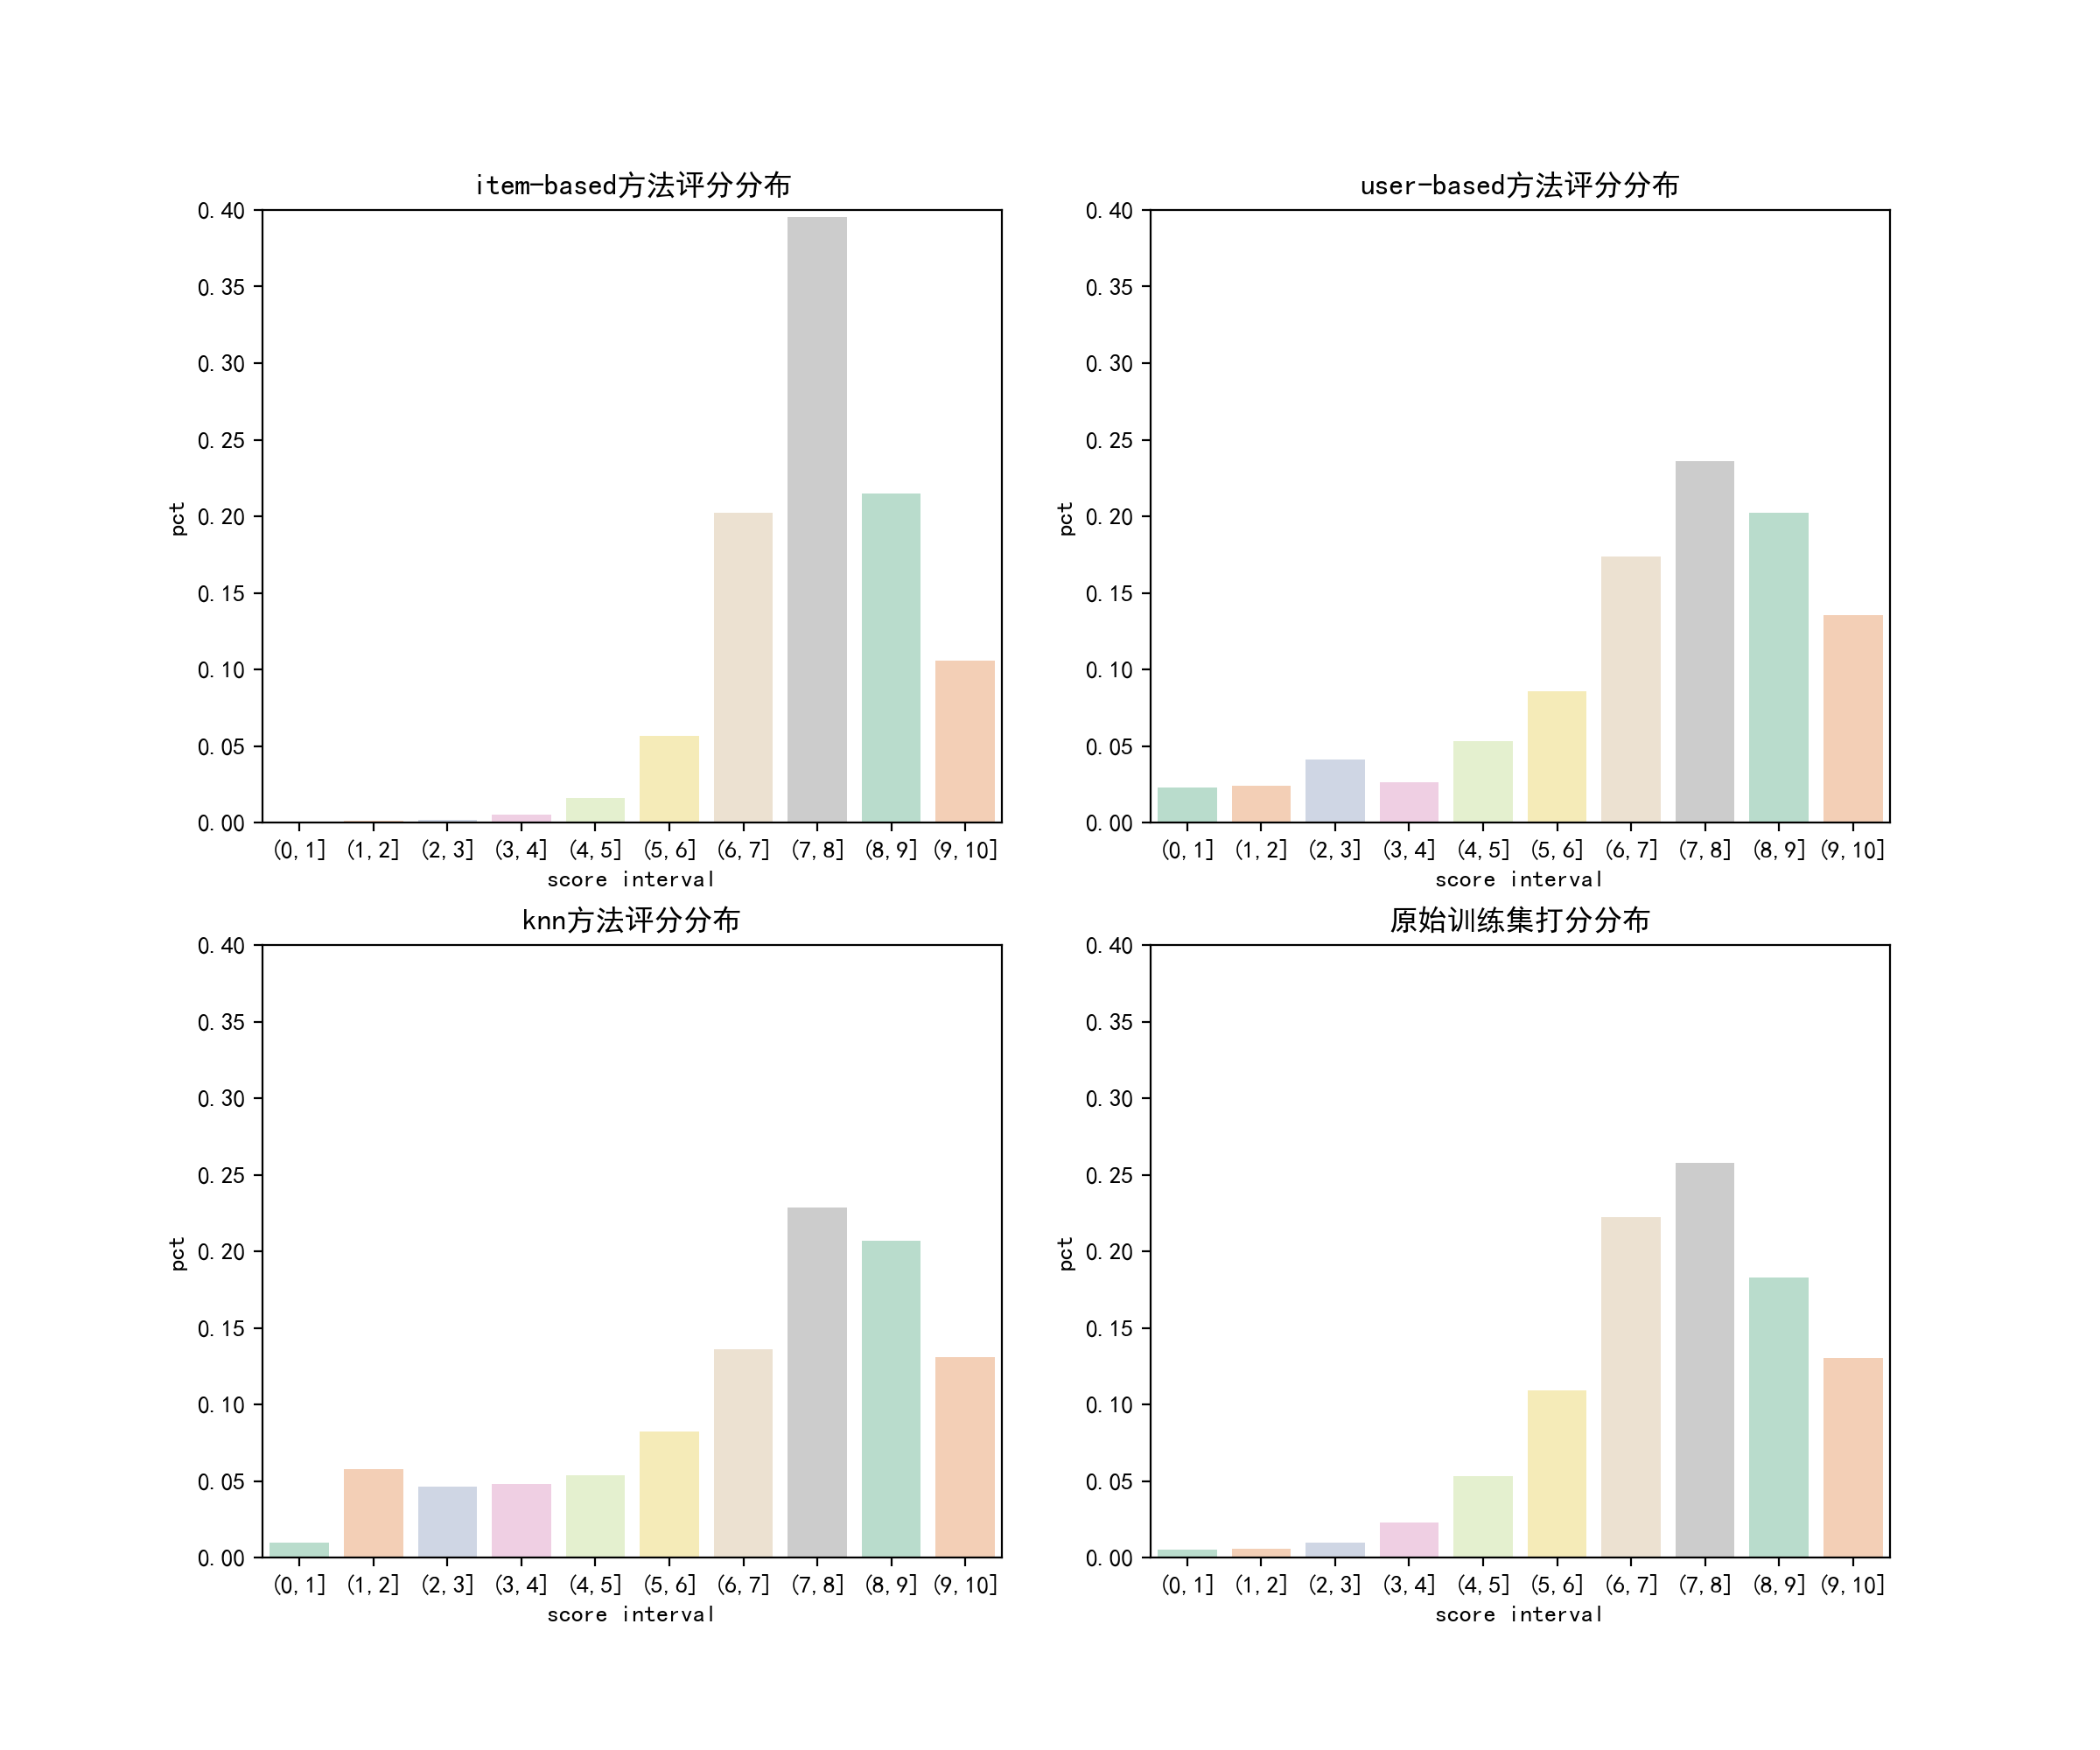
\includegraphics[height=12.0cm,width=16.0cm]{figure/pred_score.png}
	\caption{三种填充方法各自预测评分结果的分布情况}
	\label{fig: pred_score_distribution}
\end{figure}

表~\ref{tab:missing_imputation_results_3}是用KNN填充以及上述两种基于领域的方法对样本得分填充后,四种召回算法在测试集上的效果对比:
% Table generated by Excel2LaTeX from sheet 'imputation'
\begin{table}[htbp]
	\centering
	\caption{三种缺失填充方法结果对比}
	%\textbf{表4.11}~~三种填充方法比较
	\resizebox{\textwidth}{!}{
		\begin{tabular}{rlrrrrrrrr}
			\toprule
			&      & \multicolumn{4}{c}{K=10}  & \multicolumn{4}{c}{K=20} \\
			\cmidrule{3-10}    \multicolumn{1}{l}{Algorithm} & Imputation & \multicolumn{1}{l}{Recall} & \multicolumn{1}{l}{Precision} & \multicolumn{1}{l}{Hit\_rate} & \multicolumn{1}{l}{Coverage} & \multicolumn{1}{l}{Recall} & \multicolumn{1}{l}{Precision} & \multicolumn{1}{l}{Hit\_rate} & \multicolumn{1}{l}{Coverage} \\
			\midrule
			\multicolumn{1}{l}{Item\_CF} & none & 2.148\% & 10.394\% & 44.700\% & 13.107\% & 3.778\% & 9.190\% & 55.744\% & 18.386\% \\
			& knn  & 2.272\% & \textbf{10.947\%} & 45.546\% & \textbf{13.572\%} & 3.981\% & \textbf{9.633\%} & 57.638\% & \textbf{20.771\%} \\
			& user & 2.244\% & 10.842\% & 45.546\% & 13.317\% & 3.931\% & 9.535\% & 56.711\% & 20.441\% \\
			& item & \textbf{2.284\%} & 10.840\% & \textbf{46.030\%} & 13.182\% & \textbf{4.044\%} & 9.618\% & \textbf{58.847\%} & 19.811\% \\
			\multicolumn{1}{l}{Item\_related} & none & 1.466\% & 7.247\% & 35.953\% & 22.615\% & 2.656\% & 6.770\% & 48.609\% & 27.070\% \\
			& knn  & 1.569\% & \textbf{7.728\%} & 38.210\% & 22.451\% & 2.807\% & 7.110\% & 49.980\% & 26.785\% \\
			& user & 1.541\% & 7.609\% & 37.565\% & 22.376\% & 2.817\% & \textbf{7.163\%} & 50.181\% & 26.920\% \\
			& item & \textbf{1.585\%} & 7.648\% & \textbf{38.613\%} & \textbf{22.466\%} & \textbf{2.866\%} & 7.108\% & \textbf{51.270\%} & \textbf{26.965\%} \\
			\multicolumn{1}{l}{gender+age} & none & 2.036\% & 9.177\% & 41.999\% & 3.824\% & 3.641\% & 8.230\% & 52.358\% & 5.324\% \\
			& knn  & \textbf{2.104\%} & \textbf{9.482\%} & \textbf{42.805\%} & \textbf{3.839\%} & \textbf{3.715\%} & \textbf{8.378\%} & 53.446\% & \textbf{5.849\%} \\
			& user & 2.093\% & 9.434\% & 42.523\% & 3.719\% & 3.665\% & 8.267\% & 52.842\% & 5.774\% \\
			& item & 2.075\% & 9.348\% & 42.563\% & 3.764\% & 3.684\% & 8.306\% & \textbf{53.567\%} & 5.849\% \\
			\multicolumn{1}{l}{Item\_similarity} & none & 2.438\% & 11.002\% & 48.408\% & 4.874\% & 4.350\% & 9.866\% & 58.081\% & 5.549\% \\
			& knn  & 2.462\% & 11.106\% & 48.811\% & \textbf{4.769\%} & 4.326\% & 9.796\% & 59.008\% & \textbf{5.579\%} \\
			& user & 2.455\% & 11.072\% & 48.771\% & 4.784\% & \textbf{4.352\%} & 9.849\% & 59.008\% & 5.564\% \\
			& item & \textbf{2.499\%} & \textbf{11.256\%} & \textbf{49.496\%} & 4.694\% & 4.348\% & \textbf{9.815\%} & \textbf{58.726\%} & 5.534\% \\
			\bottomrule
	\end{tabular}}%
	\label{tab:missing_imputation_results_3}%
\end{table}%

从结果上看,三种填充方法都对召回算法的结果有改善。具体地,knn方法对人口统计召回的提升效果比较好,基于物品邻域的评分预测对剩余的三种召回算法提升较大,而基于用户邻域的评分预测方法相对上述两种方法效果不是那么显著。

\section{隐反馈特征的利用}
在第3.3节正负样本构造中,提到了怎样设置训练集和测试集的样本标签,当时的做法是为my\_score特征统一给定一个阈值,打分高于阈值的样本标签$y=1$,打分低于阈值的样本标签$y=0$,阈值的设定等于8分。但是这么做的话,数据集中其他一些与“用户是否喜欢该动漫”有联系的隐反馈特征就没有用上,因此综合考虑隐反馈特征和显反馈特征(打分)来决定样本标签应该会使得推荐效果更好。本节考虑如下两个隐反馈特征:my\_watched\_episodes(用户观看的集数)和my\_status(用户观看状态)。
\subsection{结合观看集数来设置样本标签}
对于训练集中的某一个样本,如果用户在打分时所观看的集数占该动漫总集数的比例越大,理应认为其对应的打分信息的可信程度越高,因此在设置样本标签时可以在原有的my\_score阈值基础上引入一个新的条件,即:用户观看集数/动漫总集数的比例大小,并同样给定一个阈值ratio。如果打分大于等于8分并且观看集数比例大于ratio时,$y=1$,否则$y=0$:
\begin{equation}
y=\begin{cases}
1 & my\_score\geq 8\;\;\textbf{and} \frac{my\_watched\_episodes}{episodes}\geq ratio \\
0 & \textbf{else}
\end{cases}
\end{equation}

原始数据集中存在少量的动漫,其episodes=0。由于我们想要通过用户观看集数/动漫总集数这个比例来构造样本标签,分母显然不能为零,因此要对这一部分的数据进行缺失值填充。填充的方法比较简单,就是用训练集中该动漫对应的所有样本里,my\_watched\_episodes特征取值的最大值代替(用用户已经看过的集数的最大值来作为总集数的估计)。表~\ref{tab:watched_ratio_results}是结合了观看集数比例设置样本标签后各组召回算法的效果,以及最后xgb精排后的结果。
% Table generated by Excel2LaTeX from sheet 'watched'
\begin{table}[htbp]
	\centering
	\caption{结合用户观看集数比例构造标签后的推荐结果}
	%\textbf{表4.12}~~考虑用户观看集数比例后的推荐效果
	\resizebox{\textwidth}{!}{
		\begin{tabular}{rlrrrr}
			\toprule
			\multicolumn{1}{l}{ratio\_threshold} & Algorithm & \multicolumn{1}{l}{Recall} & \multicolumn{1}{l}{Precision} & \multicolumn{1}{l}{Hit\;rate} & \multicolumn{1}{l}{Coverage} \\
			\midrule
			0    & \textbf{gender+age} & \textbf{3.641\%} & \textbf{8.230\%} & \textbf{52.358\%} & \textbf{5.324\%} \\
			0.5  & gender+age & 3.595\% & 8.126\% & 51.794\% & 5.339\% \\
			0.6  & gender+age & 3.591\% & 8.118\% & 51.673\% & 5.339\% \\
			0.7  & gender+age & 3.580\% & 8.092\% & 51.632\% & 5.339\% \\
			0.8  & gender+age & 3.568\% & 8.066\% & 51.552\% & 5.354\% \\
			0    & \textbf{Item-related} & \textbf{1.466\%} & \textbf{7.247\%} & \textbf{35.953\%} & \textbf{22.615\%} \\
			0.5  & Item-related & 1.543\% & 7.657\% & 37.525\% & 22.660\% \\
			0.6  & Item-related & 1.556\% & 7.724\% & 37.888\% & 22.466\% \\
			0.7  & Item-related & 1.543\% & 7.662\% & 37.646\% & 22.555\% \\
			0.8  & Item-related & 1.554\% & 7.722\% & 38.170\% & 22.376\% \\
			0    & \textbf{Item-CF} & \textbf{3.778\%} & \textbf{9.190\%} & \textbf{55.744\%} & \textbf{18.386\%} \\
			0.5  & Item-CF & 3.739\% & 9.104\% & 55.542\% & 21.056\% \\
			0.6  & Item-CF & 3.751\% & 9.133\% & 55.462\% & 21.101\% \\
			0.7  & Item-CF & 3.744\% & 9.118\% & 55.421\% & 21.131\% \\
			0.8  & Item-CF & 3.730\% & 9.084\% & 55.139\% & 21.251\% \\
			0    & \textbf{Item-similarity} & \textbf{4.208\%} & \textbf{9.498\%} & \textbf{57.517\%} & \textbf{5.624\%} \\
			0.5  & Item-similarity & 4.319\% & 9.800\% & 58.525\% & 5.759\% \\
			0.6  & Item-similarity & 4.320\% & 9.805\% & 58.565\% & 5.729\% \\
			0.7  & Item-similarity & 4.316\% & 9.795\% & 58.565\% & 5.729\% \\
			0.8  & Item-similarity & 4.331\% & 9.830\% & 58.525\% & 5.729\% \\
			0    & \textbf{xgboost} & \textbf{7.469\%} & \textbf{11.203\%} & \textbf{77.872\%} & \textbf{21.296\%} \\
			0.5  & xgboost & 7.587\% & 11.392\% & 77.711\% & 24.280\% \\
			0.6  & xgboost & 7.575\% & 11.388\% & 77.348\% & 23.635\% \\
			0.7  & xgboost & 7.566\% & 11.361\% & 77.872\% & 23.410\% \\
			0.8  & xgboost & 7.549\% & 11.336\% & 77.227\% & 23.815\% \\
			\bottomrule
	\end{tabular}}%
	\label{tab:watched_ratio_results}%
\end{table}%

从表~\ref{tab:watched_ratio_results}可以得到:
\begin{itemize}
	\item 设置了ratio阈值后,Item-related召回和Item-similarity召回的结果都有比较明显的提升;人口统计召回和Item-based CF召回效果略微下降
	\item 设置了ratio阈值后,经过xgboost重排后的结果也比之前有了提高,相对来说,ratio阈值较低时,重排后的结果会更好一些。
\end{itemize}

所以将特征my\_watched\_episodes纳入样本标签构造的规则中是有显著作用的。

\subsection{结合观看状态来设置样本标签}
表~\ref{tab:status_score_distribution}有统计过不同的my\_status对应用户打分的分布情况,很明显地可以看出:不同的my\_status对应的打分分布是有差异的,因此之前设置label时候所用的统一给定一个阈值的方法并不是十分的合理,不同的my\_status取值$i$应当对应一个不同的阈值$t_i$。另一方面,各状态样本所占全体样本的比例也不一样,显然对于样本数越多的状态,其不同的阈值选取对结果带来的影响也越大。在整个训练集中,最多的completed状态非零打分样本($my\_status=2$)占所有非零打分训练样本的$89\%$,而最少的plan to watch状态非零打分样本仅占$0.004\%$。下面是对各状态的阈值变化对应推荐效果变化的探索结果(类似于grid-search,更多的具体结果详见附件):

\begin{enumerate}
	\item $my\_status=2$:令$t_2\in\{7,8,9\}$,其余状态阈值为:$t_1\in\{7,8,9\},\;\;t_3\in\{7,8\},\;\;t_4=8$,这样一共可以比较六组实验的最终结果,表~\ref{tab:status=2}是其中一组的结果(阈值分别为$t_1=8,\;t_3=8,\;t_4=8$,即之前默认的统一阈值取值。)。可以看出:$t_2=8$时的最终推荐效果,要显著优于其$t_2=7\;\text{or}\;9$时的效果。
	% Table generated by Excel2LaTeX from sheet 'status=2'
	\begin{table}[htbp]
		\centering
		\caption{my\_status=2对应不同阈值下的推荐结果}
		%\textbf{表4.13}~~ my\_status=2的阈值变化结果
		\resizebox{\textwidth}{!}{
			\begin{tabular}{rlrrrr}
				\toprule
				\multicolumn{1}{l}{threshold} & Algorithm & \multicolumn{1}{l}{Recall} & \multicolumn{1}{l}{Precision} & \multicolumn{1}{l}{Hit\;rate} & \multicolumn{1}{l}{Coverage} \\
				\midrule
				7    & gender+age & 3.510\% & 7.932\% & 50.988\% & 5.369\% \\
				8    & \textbf{gender+age} & \textbf{3.641\%} & \textbf{8.230\%} & \textbf{52.358\%} & \textbf{5.324\%} \\
				9    & gender+age & 3.722\% & 8.417\% & 54.373\% & 5.339\% \\
				7    & Item-related & 1.489\% & 7.303\% & 36.638\% & 22.705\% \\
				8    & \textbf{Item-related} & \textbf{1.466\%} & \textbf{7.247\%} & \textbf{35.953\%} & \textbf{22.615\%} \\
				9    & Item-related & 1.418\% & 7.302\% & 34.865\% & 22.271\% \\
				7    & Item-CF & 3.577\% & 8.686\% & 53.648\% & 21.371\% \\
				8    & \textbf{Item-CF} & \textbf{3.778\%} & \textbf{9.190\%} & \textbf{55.744\%} & \textbf{18.386\%} \\
				9    & Item-CF & 3.770\% & 9.224\% & 58.565\% & 26.770\% \\
				7    & Item-similarity & 4.423\% & 10.022\% & 58.888\% & 5.474\% \\
				8    & \textbf{Item-similarity} & \textbf{4.208\%} & \textbf{9.498\%} & \textbf{57.517\%} & \textbf{5.624\%} \\
				9    & Item-similarity & 4.072\% & 9.264\% & 56.993\% & 5.759\% \\
				7    & xgboost & 7.340\% & 11.021\% & 77.106\% & 22.735\% \\
				8    & \textbf{xgboost} & \textbf{7.469\%} & \textbf{11.203\%} & \textbf{77.872\%} & \textbf{21.296\%} \\
				9    & xgboost & 7.385\% & 11.092\% & 77.194\% & 26.110\% \\
				\bottomrule
		\end{tabular}}%
		\label{tab:status=2}%
	\end{table}%
	
	\item $my\_status=1$:令$t_1\in\{7,8,9\}$,其余状态阈值为:$t_3\in\{7,8\},t_2=t_4=8$,从表~\ref{tab:status=1}可以看出:$t_1=9$时的最终推荐效果略优
	% Table generated by Excel2LaTeX from sheet 'status=1'
	\begin{table}[htbp]
		\centering
		\caption{my\_status=1对应不同阈值下的推荐结果}
		%\textbf{表4.14}~~my\_status=1的阈值变化结果
		\resizebox{\textwidth}{!}{
			\begin{tabular}{rlrrrr}
				\toprule
				&      & \multicolumn{1}{l}{t\_3=8} &      & \multicolumn{1}{l}{t\_3=7} &  \\
				\cmidrule{3-6}    \multicolumn{1}{l}{threshold} & Algorithm & \multicolumn{1}{l}{Recall} & \multicolumn{1}{l}{Precision} & \multicolumn{1}{l}{Recall} & \multicolumn{1}{l}{Precision} \\
				\midrule
				7    & gender+age & 3.642\% & 8.234\% & 3.647\% & 8.244\% \\
				8    & gender+age & 3.641\% & 8.230\% & 3.641\% & 8.230\% \\
				9    & gender+age & 3.624\% & 8.193\% & 3.622\% & 8.188\% \\
				7    & Item-related & 1.466\% & 7.244\% & 1.477\% & 7.285\% \\
				8    & Item-related & 1.466\% & 7.247\% & 1.470\% & 7.258\% \\
				9    & Item-related & 1.474\% & 7.296\% & 1.469\% & 7.258\% \\
				7    & Item-CF & 3.772\% & 9.170\% & 3.766\% & 9.153\% \\
				8    & Item-CF & 3.778\% & 9.190\% & 3.736\% & 9.082\% \\
				9    & Item-CF & 3.708\% & 9.017\% & 3.714\% & 9.030\% \\
				7    & Item-similarity & 4.323\% & 9.804\% & 4.370\% & 9.909\% \\
				8    & Item-similarity & 4.208\% & 9.498\% & 4.361\% & 9.890\% \\
				9    & Item-similarity & 4.332\% & 9.829\% & 4.341\% & 9.848\% \\
				7    & xgboost & 7.453\% & 11.181\% & 7.437\% & 11.167\% \\
				8    & xgboost & 7.469\% & 11.203\% & 7.447\% & 11.182\% \\
				9    & xgboost & \textbf{7.523\%} & \textbf{11.296\%} & \textbf{7.533\%} & \textbf{11.311\%} \\
				\bottomrule
		\end{tabular}}%
		\label{tab:status=1}%
	\end{table}%
	
	\item $my\_status=4$:令$t_4\in\{5,6,7,8\}$,其余状态阈值为:$t_1=9,\;t_2=t_3=8$。从表~\ref{tab:status=4}可以看出:$t_4\geq 6$时的模型效果都优于原始模型的效果,而当$t_4\leq 5$后,有一个显著的下滑,因此适当的阈值选取应该在6分及以上。
	% Table generated by Excel2LaTeX from sheet 'status=4'
	\begin{table}[htbp]
		\centering
		\caption{my\_status=4对应不同阈值下的推荐结果}
		%\textbf{表4.15}~~my\_status=4的阈值变化结果
		\resizebox{\textwidth}{!}{
			\begin{tabular}{rlrrrr}
				\toprule
				\multicolumn{1}{l}{988x} & Algorithm & \multicolumn{1}{l}{Recall} & \multicolumn{1}{l}{Precision} & \multicolumn{1}{l}{Hit\;rate} & \multicolumn{1}{l}{Coverage} \\
				\midrule
				5    & gender+age & 3.640\% & 8.228\% & 52.559\% & 5.354\% \\
				6    & gender+age & 3.639\% & 8.226\% & 52.439\% & 5.324\% \\
				7    & gender+age & 3.628\% & 8.201\% & 52.358\% & 5.309\% \\
				8    & gender+age & 3.624\% & 8.193\% & 52.277\% & 5.309\% \\
				5    & Item-related & 1.478\% & 7.293\% & 36.518\% & 22.406\% \\
				6    & Item-related & 1.469\% & 7.262\% & 36.195\% & 22.645\% \\
				7    & Item-related & 1.477\% & 7.305\% & 36.195\% & 22.481\% \\
				8    & Item-related & 1.474\% & 7.296\% & 36.034\% & 22.451\% \\
				5    & Item-CF & 3.726\% & 9.057\% & 55.341\% & 20.711\% \\
				6    & Item-CF & 3.710\% & 9.020\% & 55.099\% & 21.071\% \\
				7    & Item-CF & 3.719\% & 9.041\% & 55.462\% & 21.251\% \\
				8    & Item-CF & 3.708\% & 9.017\% & 55.139\% & 21.326\% \\
				5    & Item-similarity & 4.344\% & 9.855\% & 58.807\% & 5.654\% \\
				6    & Item-similarity & 4.340\% & 9.847\% & 58.605\% & 5.654\% \\
				7    & Item-similarity & 4.332\% & 9.829\% & 58.605\% & 5.654\% \\
				8    & Item-similarity & 4.332\% & 9.829\% & 58.726\% & 5.714\% \\
				5    & xgboost & 7.457\% & 11.197\% & 78.517\% & 22.076\% \\
				6    & xgboost & 7.518\% & 11.290\% & 78.033\% & 22.780\% \\
				7    & xgboost & 7.531\% & 11.309\% & 78.275\% & 22.211\% \\
				8    & xgboost & 7.523\% & 11.296\% & 77.993\% & 22.825\% \\
				\bottomrule
		\end{tabular}}%
		\label{tab:status=4}%
	\end{table}%
\end{enumerate}

综上所述,除了$my\_status=2$的阈值选取对各召回算法效果以及最终排序结果有比较明显的影响外,其他$my\_status$的阈值改变对结果的影响其实比较微弱。这很大程度上是因为样本的$my\_status$特征取值极其不平衡,所以占据极大比重的状态2的阈值选取才是最关键的。但是如果数据集的组成有类似的隐式特征,同时类别比较均衡的时候,根据不同类设置不同阈值应该会起到更明显的作用。